\chapter{序論} % 章のタイトル

% \includegraphics[width=??cm]{hoge.eps} % 図(EPS形式)を読み込む場合

\section{背景} % sectionのタイトル

% 以下に背景,関連する環境状況,技術に関する概要を記述.

近年,インターネット技術やセンサー技術の進化を背景に,パソコンやスマートフォンなどのインターネット端末に加え,家電や自動車などの様々なものに通信機能を搭載したIoTデバイスが普及し始めている.総務省によると世界中のIoTデバイスの数は図\ref{fig:IoT}のように2017年時点でIoTデバイスが約275億台存在し,2020年にはIoTデバイスが403億台に及ぶと予想されている\cite{IoT}.
 \begin{figure}[hb]
 \centering
    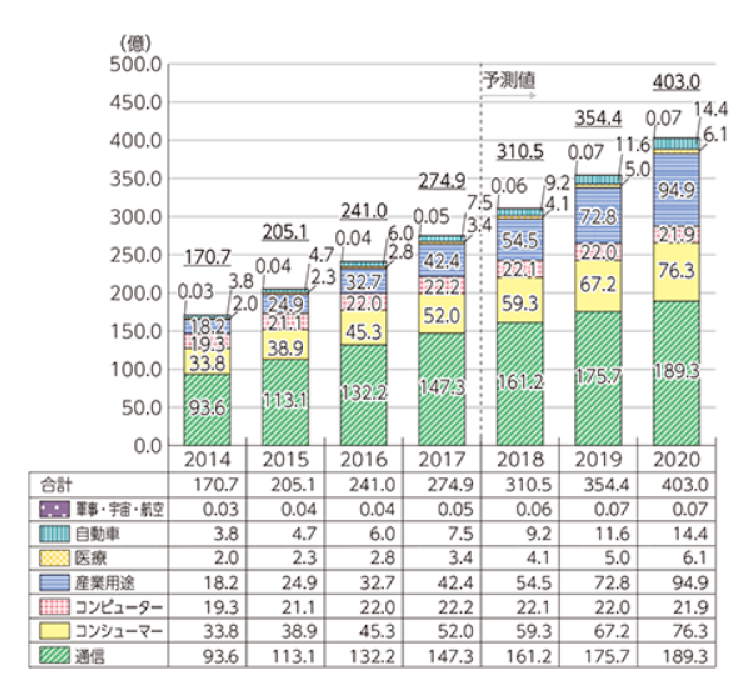
\includegraphics{figures/IoT_device.eps}
    \caption{世界のIoTデバイス数の推移及び予測(平成30年版情報通信白書\cite{IoT}より引用)}
 \label{fig:IoT}
 \end{figure}
 \clearpage
%参考文献を入れ直す
%タイトルに"(~~より引用)"を付け加える.

IoTデバイスを対象としたマルウェアが急増している.
IoTデバイスの普及に伴う重要な問題の1つとしてセキュリティ問題が挙げられる.IoTデバイスのユーザ名やパスワードを初期設定の状態で使用する場合が多いことや,デバイスの資源が限られていることから,セキュリティが十分に考慮されていないことがある.そのため,IoTデバイスを対象としたマルウェアが脅威となっている.その中でもネットワークサービスを停止させる深刻な問題を引き起こしているマルウェアにはDDoS(Distributed Denial of Service)攻撃を行っているものが多く存在し,その対策が重要視されている.DDoS攻撃は,複数の他人のコンピュータを攻撃者が悪用し,公開されているサービスに大量のデータを送りつける事によって処理負荷を与えサービスを機能停止に追い込む攻撃である.代表的なDDoS攻撃を行うマルウェアとしてMirai\cite{Mirai}が挙げられる.\par
Miraiを利用して2016年10月に発生した,DNSサーバープロバイダであるDyn社へのDDoS攻撃ではIoTデバイスによるボットネットが利用され史上最大規模である620Gbpsの攻撃が観測された\cite{Dyn}.その後,Miraiのソースコード\cite{code}が公開され,Wicked\cite{Wicked},Satori\cite{Satori},Okiru\cite{Okiru}といったMiraiの亜種の開発が盛んに行われるようになった.2017年には,Windows PCを踏み台にして感染可能なIoTデバイスを探索するMiraiによるネットワーク活動が観測された\cite{newMirai}.このMiraiは多くの端末に感染させることを目的としており,IoTデバイスを探索する機能に特化させたMiraiとなっている.初期のMiraiよりも多くのポートをスキャンしログイン可能な端末を探索することによりMiraiを様々なIoTデバイスに拡散させることが可能になっている.MiraiやMirai亜種のマルウェアによって,多くのIoTデバイスがDDoS攻撃に不正利用されることから,国立研究開発法人情報通信研究機構がパスワード設定などに不備のあるIoT機器の実態把握を目的として日本国内のIPv4アドレスを対象にSSH,Telnet,HTTPであるTCPの22番,23番,80番ポートを対象にポートスキャンを行った\cite{国立}.これらの事例から,IoTデバイスの不正利用によるDDoS攻撃が問題視されており,社会的に注目されている.

\section{IoTデバイス本体で検知を行う必要性}

IDS(Instrusion Detection System)と呼ばれるマルウェアによる不正な通信やホストへの侵入,ファイルの改ざん等の不正な挙動の兆候を検出するシステムの設置場所としてネットワーク上に設置するネットワーク型と端末上に設置するホスト型の2種類が考えられる.ネットワーク型のIDSでは,ネットワーク上に流れるデータを取得して解析し,不正と疑われるデータを検知したときには管理者に通知する.ネットワークトラフィックからDDoS攻撃を判別するのは難しく,誤検知する可能性が考えられる.しかし,ホスト型IDSにて見られる,マルウェアに基づいて作成されたデータを用いたパターンマッチングによる検知手法では,誤検知率が低く既存のマルウェアを確実に検知できる利点がある.公開されているソースコードを基に作成されたマルウェアは,オリジナルのマルウェアと共通するシグネチャが存在すると考えられるためパターンマッチングによる検知で亜種のマルウェアにも対応できると想定される.\par
脅威となっているマルウェアは,十分に管理が行われていないIoTデバイスで散見される,放置された初期パスワードのままのアカウントや,保守されていないシステムの脆弱性をついた攻撃を行うため,侵入されてしまうことは前提とすべきである.デバイス上で検知をすることによって侵入したマルウェアによる不正な挙動の痕跡からパターンマッチングによる検知を行うことができる.そのため,デバイスの性能が限られているIoTデバイス上でマルウェアの検知を行う必要がある.

%なぜ本体で検知を行うのか書く必要がある
\section{マルウェア解析}
%マルウェアの検体を保持していることを前提に説明しているのでその説明をする.
マルウェア解析とは,端末上にダウンロードされたマルウェアから内在している情報を得るための行為である.例えば,マルウェアが具備している機能を明らかにしたり,どの組織を狙っているのか,マルウェアが作成された目的を明らかにするために行われる.マルウェア解析には,表層解析,動的解析,静的解析の3つのプロセスが存在している\cite{実践}.表層解析は,ファイル自体が悪性であるかどうかの情報収集や,ファイルのメタ情報の収集を行う.ファイルタイプや動作するCPUアーキテクチャの情報,ハッシュ値などをもとに,既知のマルウェアかどうか判定を行う.表層解析では,解析対象に対して解析ツールを用いて情報を収集する.マルウェアを動作させたり,マルウェア内のプログラムコードを分析したりはしない.動的解析は,マルウェアが実際に動作した際に端末上にどのような痕跡が残るのか,またどのような通信が発生するのかの情報収集を行う.ファイルやレジストリアクセスの情報を収集したり,通信を監視して通信先のIPアドレスやドメイン,URL,通信ペイロードといった情報を収集する.マルウェアを動作させるため,動的解析を行う環境は図\ref{fig:env}のように通常利用しているホストやネットワークから隔離しておくなど,安全性に対する十分な配慮が必要である.静的解析は,逆アセンブラやデバッガを用いてマルウェアのプログラムコードを分析し,具備されている機能や特徴的なバイト列など詳細な情報を収集する.動的解析で実行されなかったコードを分析して潜在的に保有している機能を明らかにしたり,マルウェア独自の通信プロトコルや通信先生成アルゴリズムのような動的解析だけでは特定が難しい情報の収集を行う.IoTデバイス上でマルウェアと判別するためには,疑わしいファイルを解析する必要がある.しかし,資源の限られたIoTデバイス上で静的解析を行い,疑わしいファイルをデバッガなどを用いてプログラムコードからマルウェアと判別する手法では,デバッガなどがIoTデバイス本来の動作を阻害してしまう可能性が高い.そのため,疑わしいファイルを解析する方法として動的解析や表層解析が候補として挙げられる.

\newpage

\begin{figure}[h]
   \centering
      \includegraphics[width=100mm]{figures/env.eps}
      \caption{動的解析環境}
   \label{fig:env}   
\end{figure}

\begin{figure}[h]
   \centering
      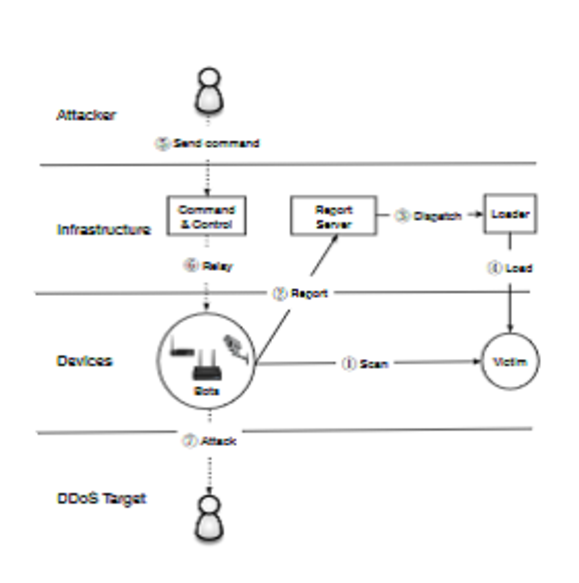
\includegraphics[width=100mm]{figures/s.eps}
      \caption{Miraiの概要図}
   \label{fig:Mirai_system}   
\end{figure}

 

\section{マルウェアMiraiの概要}

Miraiは,ネットワーク上で公開されているLinuxで動作するデバイスを不正利用し,DDoS攻撃を行うマルウェアである.ネットワークカメラやルータといったIoTデバイスをターゲットにしている.Miraiは,C\&Cサーバー,攻撃対象の管理データベース,Loader,botの4つから構成される.Miraiの概要を図\ref{fig:Mirai_system}に示す.

%新しいものを入れる.

C\&Cサーバーは,ボットやユーザーから接続されるのを待機しており,主な機能としてボット管理機能,ユーザー管理機能,攻撃指示機能がある.攻撃対象の管理データベースとしてMySQLが利用されており,ユーザーのリストと攻撃履歴が記録されるようになっている.botは,C\&Cサーバーからの攻撃命令を待機し,感染先でボットネットに加えられる新しいデバイスを探索するスキャン活動を行う.スキャン活動を行いログインできる端末を見つけた場合には,IPアドレス,ポート,ログイン情報をスキャンサーバーへと送る.Miraiは、Telnetログインが可能な場合に感染する.Loaderは,スキャン活動からレポートサーバーに送られた端末のログイン情報をもとにTelnetログインを試みる.Telnetログインに成功した際には,攻撃者が用意したhttpサーバーまたはtftpサーバーから,Miraiのバイナリファイルを対象のIoTデバイスにダウンロードしbotを実行させる.botの動作後には,C\&Cサーバーとの通信を始め,C\&Cサーバーから送られてくる攻撃命令を受け取り,IoTデバイスが特定のサーバーに攻撃を始める.C\&CサーバーによるDDoS攻撃命令は表\ref{tab:attack}のように10種類存在しており,攻撃を行ったbotは再びC\&Cサーバーから攻撃命令が送られてくるのを待機している.

\begin{table}[h]
   \caption{攻撃種類}
   \centering
   \label{tab:attack}
   \begin{tabular}{|l|l|}
   \hline
   攻撃種類                            & 詳細 \\ \hline \hline
   UDP攻撃                           &   UDPパケットを大量に送信する \\ \hline
   プレーンUDP攻撃                    & 高速化のために最適化を行いUDPパケットを大量に送信する   \\ \hline
   SYN攻撃                           &  SYNパケットを大量に送信する  \\ \hline
   ACK攻撃                           &  ACKパケットを大量に送信する  \\ \hline
   HTTP攻撃                          &  HTTPリクエストを大量に送信する  \\ \hline
   DNSリゾルバ攻撃                       &  DNSサーバーへ大量の名前解決のためのリクエストを送信する  \\ \hline
   GRE IP 攻撃                       &  GREプロトコルによるパケットを大量に送信する  \\ \hline
   GREイーサネット攻撃                     &  イーサネットとGREプロトコルによるパケットを大量に送信する  \\ \hline
   VSE攻撃                           &  ゲームエンジンに対してUDPパケットを大量に送信する  \\ \hline
   STOMP攻撃                         &  TCPセッション確立後にACKパケットを大量に送信する  \\ \hline
   \end{tabular}
\end{table}


\section{研究目的}
本研究の目的は,IoTデバイス上でDDoS攻撃を行うマルウェアMiraiとその亜種の未知のマルウェアの検知を行うことである.マルウェアの内部関数に着目をしたマルウェア検知手法を提案する.前項で述べたマルウェア解析方法である,表層解析,動的解析を行った2つの提案手法について述べる.表層解析を行ったマルウェア検知手法では,疑わしきバイナリファイルからシンボルテーブルと呼ばれるプログラム内で使用されている関数名,変数名を取得し,マルウェアが具備している関数の有無によってマルウェアの検出を行う.動的解析を行ったマルウェア検知手法では,マルウェアによって呼び出される内部関数によって呼び出されるシステムコール系列を用いてマルウェアの検出を行う。シンボルテーブルを用いた検知手法は,バイナリファイルのシンボルテーブルを削除するコマンドなどの検知対策が行われた場合には,マルウェアの検出をすることができない.しかし,システムコール系列を用いた検知を行うことによって,上記のような検知対策がなされた場合でもマルウェアの検出が可能になる.
%マルウェアだと疑われるバイナリファイルからシンボルテーブルと呼ばれる使用されている関数名,変数名を取得し,マルウェアが持つ独自の関数を持っていた場合に,マルウェアだと検出する.しかし,stripと呼ばれるバイナリファイルのシンボルテーブルを削除するコマンドなどの検知対策が行われた場合には,検知が行えない.マルウェアによって呼び出される内部関数によって呼び出されるシステムコール系列を用いた検知を行う事によって,検知対策がなされた場合でもマルウェアの検出が可能である.
%研究内容がシンプルすぎるのでIoTデバイス上で検知する,亜種の検知ができるとか大事な部分が抜けている.シンボルテーブルの提案手法とシステムコール呼び出し履歴を用いた手法のそれぞれの位置づけと狙いの違いを記述する.
 
\section{論文の構成}
本論文では,6章から構成されている.1章では,本研究の背景や研究目的について述べる.2章では,関連研究とその課題について述べる.3章では,シンボルテーブルを用いた検知手法の提案についてシンボルテーブルを用いたマルウェアの検出方法について述べる.4章では,システムコール呼び出し履歴を用いた検知手法について述べ,マルウェアによって呼び出されるシステムコール系列を用いたマルウェアの検出方法の課題点と解決方法について述べる.5章では,提案システムによるマルウェアの検知精度について述べ,6章でまとめる.%straceにやらせている目的や効果を記述して説明を行う.